\documentclass[onecolumn,preprintnumbers,amsmath,amssymb,superscriptaddress]{revtex4}
%\usepackage[pdftex]{graphicx}

\usepackage{amsmath,amsfonts,amssymb}
\usepackage[english]{babel}
\usepackage[latin1]{inputenc}
\usepackage[T1]{fontenc}
\usepackage{color}
\usepackage{float}
\usepackage{verbatim}
\usepackage{graphicx}
\usepackage{bm}
\usepackage{mathtools}
\usepackage{stmaryrd}
\usepackage{anyfontsize}


%\usepackage{epstopdf}
%\usepackage{array}
%\usepackage{tabularx}
%\usepackage{multirow}
\usepackage{color}
%\usepackage{multibox}
%\usepackage{rotating}
%\usepackage{lineno}
%\usepackage[left]{lineno}
%\usepackage[comma,sort&compress]{natbib}
%\usepackage{authblk}
%\usepackage{multicol}

%\bibliographystyle{ieeetr}


%\linenumbers
%\setlength\linenumbersep{3pt}

\begin{document}


%\title{Simple rules yield complex communities: deconstructed species interactions and the assembly of communities}
%\title{Community assembly and dynamics by the deconstruction of species interactions}
\title{Salmon straying description}
%\author{Justin D. Yeakel${}^{1,2,*}$, Christopher P. Kempes${}^{2}$, \& Sidney Redner${}^{2,3}$ \\ \\
%${}^1$School of Natural Science, University of California Merced, Merced, CA \\
%${}^2$The Santa Fe Institute, Santa Fe, NM \\
%${}^3$Department of Physics, Boston University, Boston MA \\
%${}^*$To whom correspondence should be addressed: jdyeakel@gmail.com
%}



\maketitle



\section*{Introduction}


\section*{Model Description}

Here we consider a local population $N_i$ and a remote population $N_j$ with a trait value $x_i$ and $x_j$ that determines the recrutiment rate for the respective population.
We assume that there is an optimum trait value $\theta_i$ and $\theta_j$ associated with each site, where recruitment is maximized if $x = \theta$.

Each population in its respective site has an optimum trait value $\theta_i$ where the rate of recruitment is maximized if $x_i = \theta_i$.

determines the recruitment rate, are assumed to be normally distributed with means $\mu_i$ and $\mu_j$ and a standard deviation $\sigma$, and are subject to selection across ecological timescales.

If there is no straying between these populations (such that they are independent), then the trait value should evolve towards the optimum ($x_i \rightarrow \theta_i$) and the recruitment rate will become maximized.
If there is straying between populations at rate $m$, then the traits in each respective location will be pulled away from the optimum, and recruitment rates will be lower, i.e. have lower fitness.
As $m$ becomes large, the populations should act as a single population.


Using the discrete population framework from Shelton and Mangel (2011), we have the following population dynamic equation for a local population $i$ and the population that is straying into it $j$.

\begin{align}
  N_i(t+1) &= \left(N_i(t) - m N_i(t) + m N_j(t) \right){\rm e}^{-Z} \\ \nonumber
  &+ \left((R_i[\mu_i(t)|\theta_i]+\tilde{P}) (N_i(t) - m N_i(t))+ (R_i[\mu_j(t)|\theta_i]+\tilde{P}) m N_j(t)\right) {\rm e}^{-\beta (N_i(t) - m N_i(t)+ m N_j(t))}
\end{align}

\noindent where the first line determines the number of individuals that survive from time $t$ to time $t+1$, and the second and third line accounts for the recruitment of individuals from the surviving population from time $t$ to time $t+1$.
Moreover, there is a demographic process error term included in the above dynamic equation, where $\tilde{P}\sim \mathcal{N}(0,s)$ where in the below example $s=0.001$

Survival: the probability of survival is ${\rm e}^{-Z}$... if $Z=0.5$ (Shelton and Mangel 2011), the probability of survival is 60\%. 
This survival probability is enacted on 1) The number of local individuals that return minus the number local individuals that stray ($N_i(t) - mN_i(t)$), in addition to the number of remote individuals that immigrate into the local patch $mN_j(t)$, and it is assumed that they all have equal probability of surviving.

Recruitment: The second line of the equation determines the recruitment from local individuals $N_i(t)-mN_i(t)$ and incoming strays $mN_j(t)$, as a function of their mean trait value at time $t$ and given the local trait optimum $\theta_i$, where the recruitment rate at low population densities is
\begin{align}
  R_i[\mu_i(t)|\theta_i] &= \int_{-\infty}^\infty r_{\rm max}\exp\left\{\frac{(x_i(t)-\theta_i)^2}{2\tau^2}\right\} {\rm pr}(x_i(t)|\mu_i,\sigma^2) {\rm d}x_i(t) \\ \nonumber
  &= \frac{r_{\rm max} \tau  }{\sqrt{\sigma ^2+\tau ^2}}\exp\left\{-\frac{(\theta_i-\mu_i(t))^2}{2 \left(\sigma ^2+\tau ^2\right)}\right\}.
\end{align}
This means that it is the mismatch between the trait mean $\mu_i(t)$ and the local optimum $\theta_i$ that determines the  growth rate at low population densities.
% The compensatory effects are then determined by the exponential, following the Ricker stock-recruitment relationship.

The third line of the equation determines recruitment from straying individuals (with density $mN_j(t)$), such that the recruitment rate is determined by the mismatch between the optimum trait value $\theta_i$ and the mean trait value of the incoming individuals $\mu_j$.

As shown above, the mean traits of both populations (the local mean trait value $\mu_i$ as well as the remote mean trait value $\mu_j$) also change through time.
Because individuals from the local population are being mixed with individuals from the remote population, the resulting trait distribution is a mixed normal.
We assume that the distribution that results after the remote and local populations are mixed together \emph{and reproduce} is normal with a mean value determined from a mixed-normal distribution and constant variance over time.
This assumption may be tested a few different ways if we deem it necessary down the road - as a first order approximation, it's probably fine.
The mean trait value thus changes through time according to the difference equation

\begin{equation}
  \mu_i(t+1) = w_i\mu_i(t) + (1-w_i)\mu_j(t) + \frac{\partial}{\partial \mu_i}\ln\left(w_i R_i[\mu_i(t)|\theta_i] + (1-w_i)R_i[\mu_j(t)|\theta_i]  \right)
  \label{eq:mu}
\end{equation}

\noindent where

\begin{equation}
  w_i=\frac{N_i(t)-m N_i(t)}{N_i(t)-m N_i(t) + m N_j(t)}.
\end{equation}

The first two factors in equation \ref{eq:mu} determine the mixed normal average of the now-mixed local and remote populations.
This mixed normal is weighted by the proportion of the population that is local and remote, respectively, which depends on the stray rate $m$.
The third part of the above equation determines how the mean trait changes through time due to natural selection (from Lande), which is proportional to the change in mean fitness with respect to the mean trait (phenotype).

You can see from the elements of the difference equations that demographics directly impact the evolution of trait means due to how the local and remote trait averages at time $t$ contribute to the trait mean at time $t+1$.

%Density dependent m



\section*{Results}

%The effects of trait evolution :: trait heritability, trait variance, and habitat heterogeneity
%% When stray rates are moderate-low, greater heritability leads to higher steady-state populations with higher PE's.
%% Lower heritability gives way to alternative stable states at lower stray rates, which become increasingly divergent
%% With habitat heterogeneity?

% Constant m
%% Fold bifurcation @ intermediate values of m
%% This bifurcation creates a region of depressed total biomass & depressed PE at increased stray rates and lower trait variances


%% PE >> 1 for low values of m
%% Spike in PE at the fold bifurcation (spike in indvidual population SD)
%% Increased environmental heterogeneity leads to spikes in PE at lower stray rates
%% Effects of heritability vs. trait variation and stable states



% Density dependent m
%% 



{\bf Initial results -- subject to to change:} As the proportion of strays increases, the average traits of both populations veer farther from their optimal values, and this results in the decline of the population steady state (because the recruitment rate is now sub-optimal for both populations). This is the nice, expected result.

The unexpected result are the alternative stable states that arise for lower values of $m$. Just where these alternative stable states arise depends on the variance as well as the difference in optimal trait values between sites ($\theta_1-\theta_2$), but you can see that this has big impacts on the portfolio effect.
Which trajectory goes to the higher or lower alternative stable state is random - an effect of the process noise injected into the system.
The change in the PE appears to be caused by large spikes in the variance of individual population trajectories where the alternative stable states begin (at the fold bifurcation).
This is a well-known phenomenon that forms the basis for early warning signals of phase transitions.

\begin{figure}[h]
\centering
\includegraphics[width=0.4\textwidth]{fig_Density.pdf}
\caption{}
\end{figure}


The differences in optimal trait values between sites ($\theta_1-\theta_2$) influence at what straying rate the alternative stable states appear.
Large differences in $\theta_1$ and $\theta_2$ can be interpreted as high environmental heterogeneity.
A cursory analysis shows that increasing environmental heterogeneity tends to lower the stray rate value $m^*$ at which the maximum PE is expected to occur.
Moreover, if the trait variance is much larger than the difference in optimal trait values between sites (such that selection is weaker), the alternative stable state phenomenon disappears, as does the spike in the portfolio effect.


\begin{figure}[h]
\centering
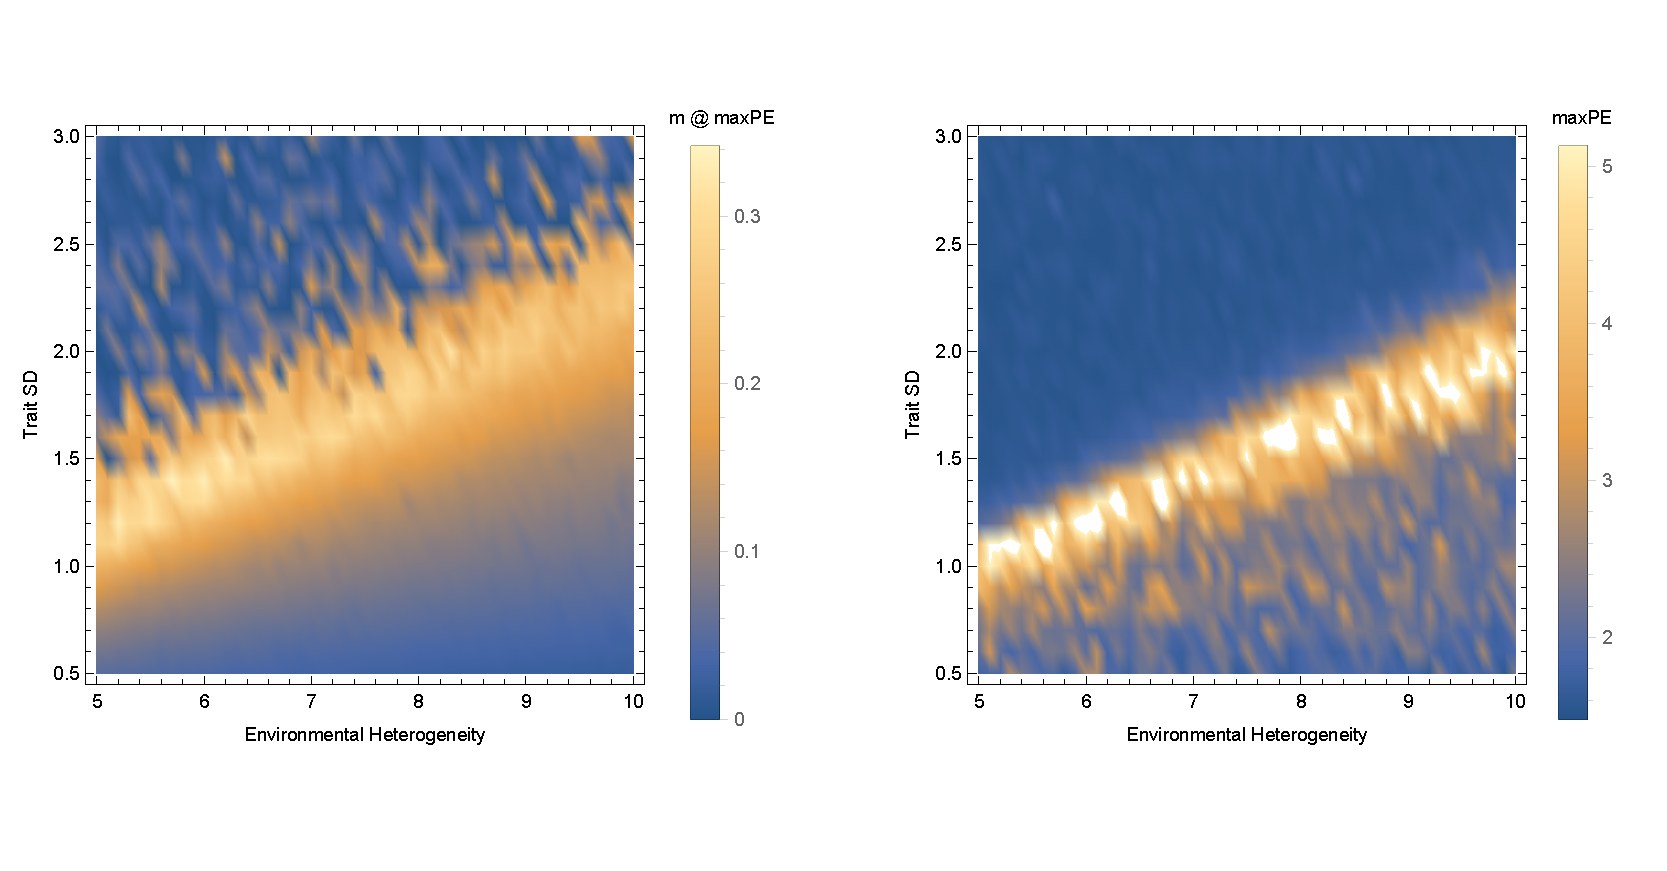
\includegraphics[width=0.8\textwidth]{fig_HSDcomb.png}
\caption{}
\end{figure}


\section*{Discussion}

\end{document}
